\documentclass[two column]{report}
\usepackage[utf8]{inputenc}

\usepackage{amsmath,amsthm,amssymb}

\usepackage{subcaption}
\usepackage{graphicx}

\usepackage{diagbox}

\usepackage{biblatex}

\bibliography{ref}

\graphicspath{{./images/}}

\usepackage{listings}


\usepackage{color}

\definecolor{gray}{rgb}{0.5,0.5,0.5}
\definecolor{orange}{rgb}{0.8,0,0}

\lstdefinestyle{matlab}{
  belowcaptionskip=1\baselineskip,
  breaklines=true,
  frame=L,
  xleftmargin=\parindent,
  language=octave,
  showstringspaces=false,
  basicstyle=\footnotesize\ttfamily,
  keywordstyle=\bfseries\color{green},
  commentstyle=\color{gray},
  identifierstyle=\color{blue},
  stringstyle=\color{orange},
}
\lstdefinestyle{R}{
  belowcaptionskip=1\baselineskip,
  breaklines=true,
  frame=L,
  xleftmargin=\parindent,
  language=R,
  showstringspaces=false,
  basicstyle=\footnotesize\ttfamily,
  keywordstyle=\bfseries\color{green},
  commentstyle=\color{gray},
  identifierstyle=\color{blue},
  stringstyle=\color{orange},
}

\def\listingsfont{\ttfamily} 
\def\listingsfontinline{\ttfamily}

\title{TAMS39 - Examination exercises}
\author{Anton Karlsson\\antka388\\931217-7117}
\date{}
\begin{document}
\maketitle

\section*{Exercise 1}

\subsection*{(a)}
\label{sec:a}

Let $H_0: \b \mu_{\rm  male} = \b \mu_{\rm female}$ against $H_{1}: \b \mu_{\rm
  male} \neq \b \mu_{\rm female}$.
We get the test statistic $T^{2}$ which is given by
\begin{equation*}
  T^{2} = n(\mean X - \b \mu_{\rm male})^{T} S^{-1}(\mean X - \b \mu_{\rm male}),
\end{equation*}
where $\b S = \frac{1}{n-1}(\b X - \b 1\mean X^{T})(\b X - \b 1\mean
X^{T})^{T}$, $\b \mu_{\rm male} = (190, 275)^{T}$, and $n$ is the size
of the population. If $p$ is the dimension of the population, then 
\begin{equation*}
  \frac{n-p}{(n-1)p}T^{2} \sim F(p,n-p+1).
\end{equation*}
A test given by rejecting $H_{0}: T^{2} \geq \frac{(n-1)p}{n-p}F_{p,
  n-p}(1 -\alpha) = c_{\alpha}$, where $\alpha = 0.05$. We get that
$c_{\alpha} \approx 6.58$ and $T^{2} \approx 5.54
$, thus we cannot reject $H_{0}$.


\subsection*{(b)}
\label{sec:b}

The confidence region is given my all $\b \mu$ such that
\begin{equation*}
  n(\mean X - \b \mu)^{T}\b S^{-1}(\mean X - \b \mu) \leq \frac{(n-1)p}{n-p}F_{p,
  n-p}(1 -\alpha) = c_{\alpha}.
\end{equation*}
The result is displayed in Figure \ref{fig:ex1-ellipse}.
\begin{figure}[h]
  \centering
  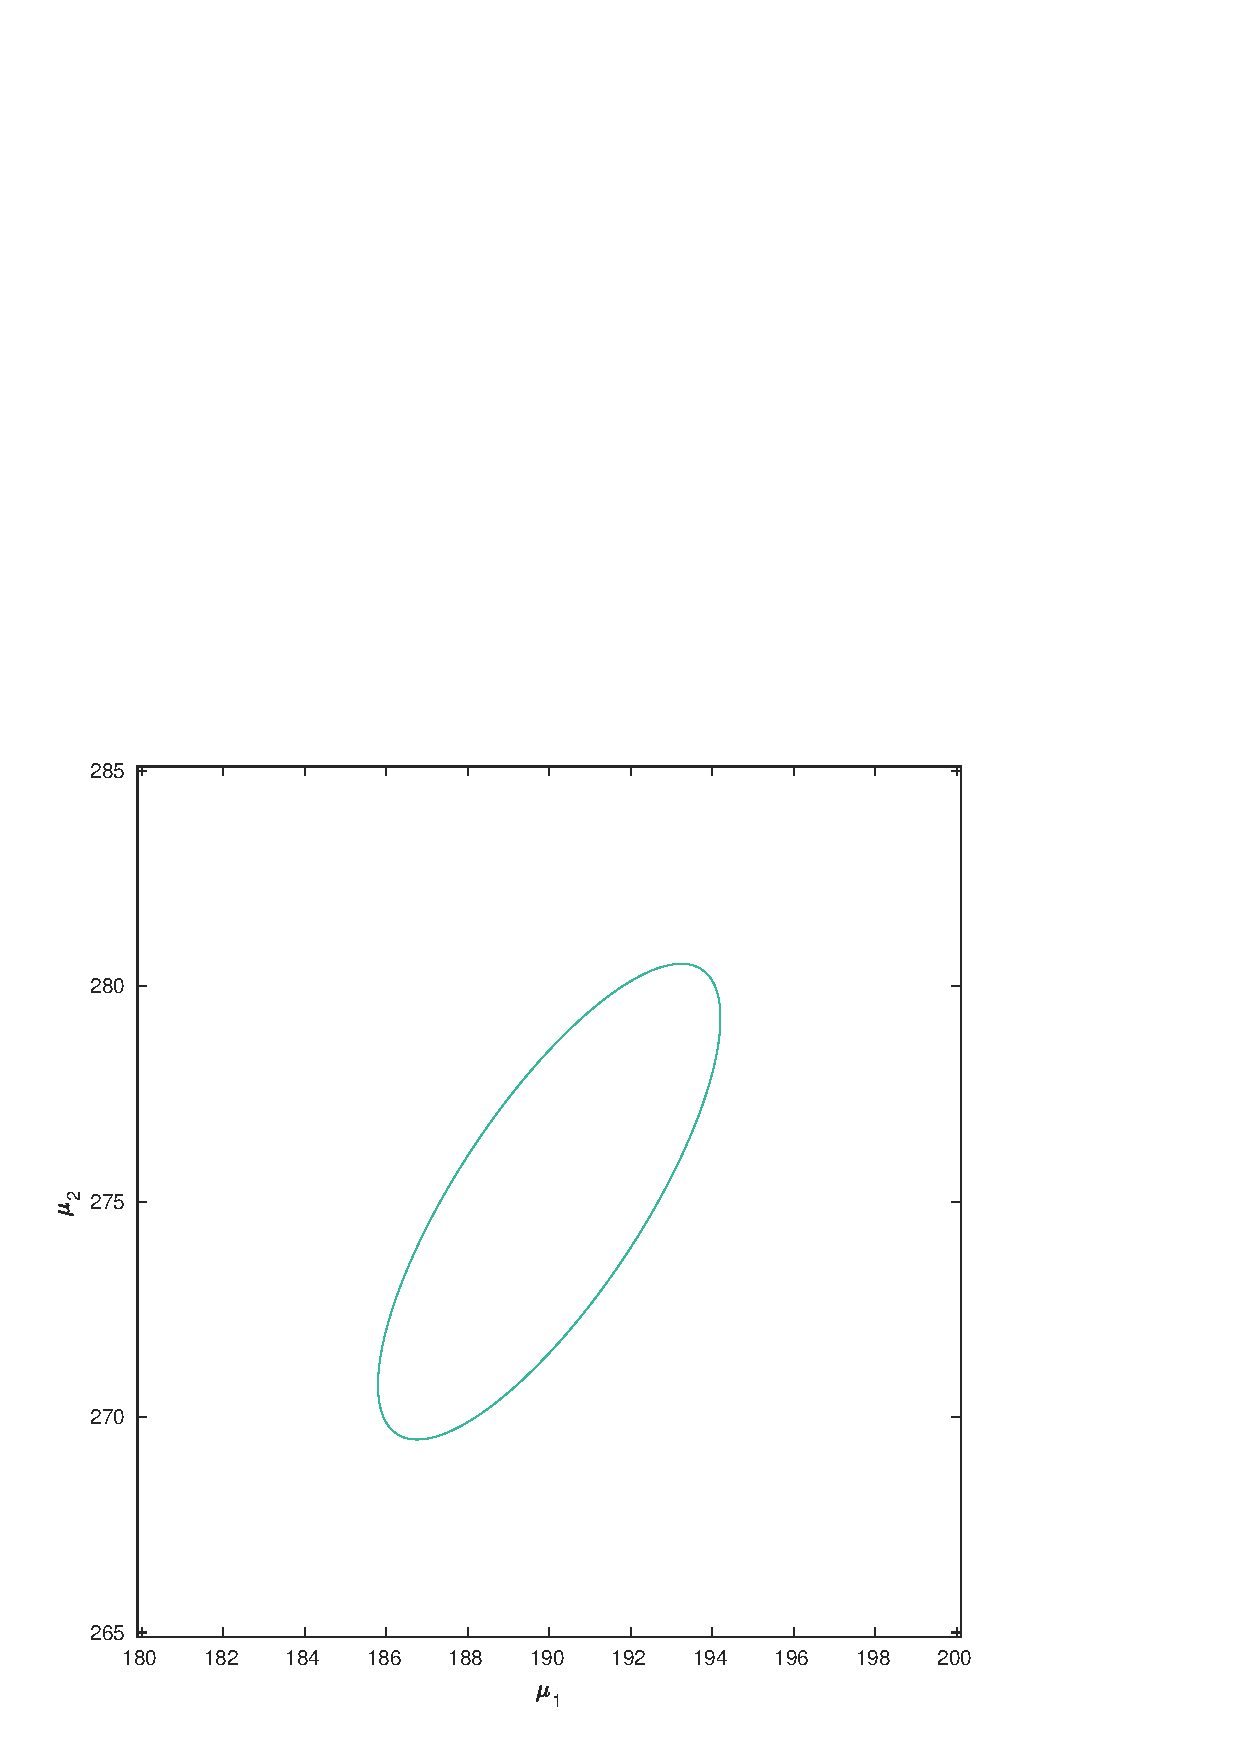
\includegraphics[width=5cm]{ellipse-ex1}
  \caption{The confidence ellipse around ${\bf \mu}$.}
  \label{fig:ex1-ellipse}
\end{figure}

\subsection*{(c)}
\label{sec:c}

From Result 5.3 in \cite[p. 225]{book} we get that simultaneously
confidence interval for $\b a' \b \mu$ is  given by
\begin{equation*}
  \b a^{T} \mean X - \sqrt{\frac{(n-1)p}{n(n-p)}F_{p,
  n-p}(1 -\alpha) \b a^{T}\b S\b a} \leq \b a^{T} \b \mu \leq 
\b a^{T} \mean X + \sqrt{\frac{(n-1)p}{n(n-p)}F_{p,
  n-p}(1 -\alpha) \b a^{T}\b S\b a} .
\end{equation*}
We get that for $\b a = (1, 0)^{T}$, which represents $\mu_{1}$, and for
$\b a = (0,1)^{T}$, which represents $\mu_{1}$, the confidence
intervals are
\begin{equation*}
  \begin{pmatrix}
    185.80 &194.20 
  \end{pmatrix},\quad \text{and} \quad
  \begin{pmatrix}
    269.48 &280.52  
  \end{pmatrix},
\end{equation*}
respectively.\\
\\
The Bonferroni intervals are given by 
\begin{equation*}
  \overline{x}_{i} \pm t_{n-1}(1 - \alpha/(2m) )\sqrt{\frac{s_{ii}}{n}},
\quad i = 1,2,
\end{equation*}
where $m= 2$ is the number of intervals. The intervals for
$\mu_{1}$ and $\mu_{2}$ are
\begin{equation*}
  \begin{pmatrix}
    186.20 &193.80 
  \end{pmatrix}, \quad \text{and}\quad
  \begin{pmatrix}
    270.00 &280.00 
  \end{pmatrix},
\end{equation*}
respectively.\\
\\
One advantage that the $T^{2}$-intervals have over the corresponding
Bonfferoni intervals is that the
Bonfferoni intervals are given by the inequaltiy
\begin{equation*}
  P\left(\text{the interval }\overline{x}_{i} \pm t_{n-1}(1 - \alpha/(2m)
  )\sqrt{\frac{s_{ii}}{n}}\text{ contains }\mu_{i},
\quad \text{for }i = 1,2,\right) \leq 1 - \alpha,
\end{equation*}
which the $T^{2}$-intervals do  not have; they have an equality
instead, meaning that the $T^{2}$-intervals can be more accurate than
the Bonfferoni intervals. 
%%% Local Variables:
%%% mode: latex
%%% TeX-master: "examination"
%%% End:

\section*{Exercise 2}
\label{sec:exercise-2}

\subsection*{(a)}
\label{sec:a-1}

The scatter plot can be found in Figure \ref{fig:ex2-scatter} the outlier can be
clearly be seen at $x_1 = 284$.
\begin{figure}[h]
  \centering
  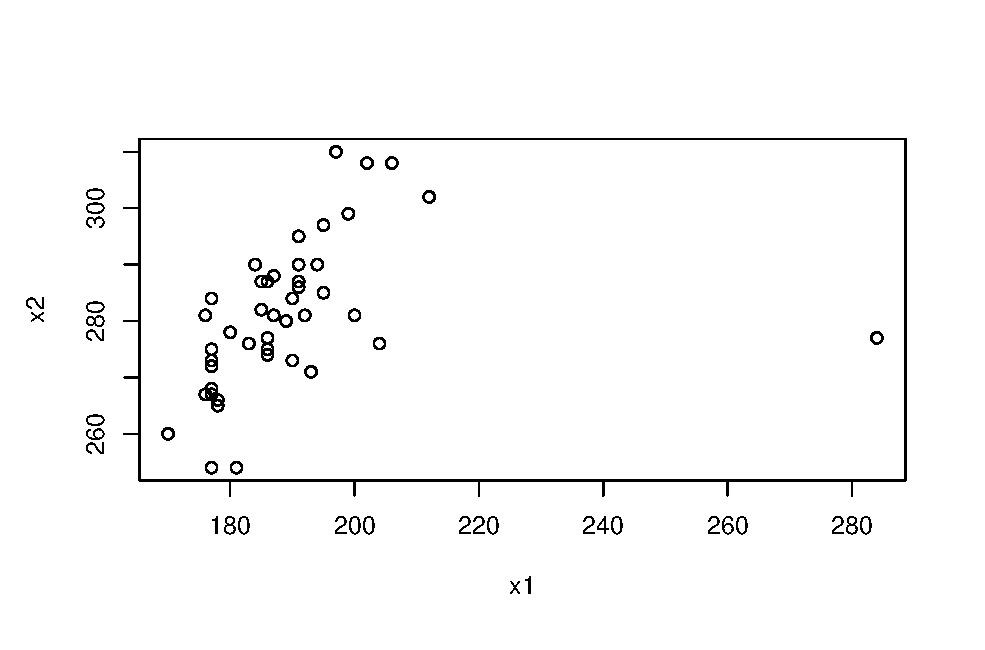
\includegraphics[width=5cm]{ex2-scatterplot}
  \caption{Scatter plot of the tail length and the wing span for male
    hook-billed kites.}
  \label{fig:ex2-scatter}
\end{figure}

\subsection*{(b)}
\label{sec:b-1}

We remove the sample with $x^{\rm male}_{1} = 284$.
Let $H_{0}: \b S_{\rm male} = \b S_{\rm female}$ versus $A \neq
H$. For this test we can use Box's test for equality of covariance
matrices, in which we reject $H_{0}$ if 
\begin{equation*}\label{eq:boxcorrection}
  (1 - u)
  \left(
    \left[
      \sum_{i=1}^{2}(n_{i} - 1)
    \right]
    \ln \abs{\b S_{\rm pooled}} - \sum_{i=1}^{2}(n_{i}-1) \ln \abs{\b S_{i}}
  \right) > \chi^{2}_{p(p+1)(g-1)/2}(1-\alpha),
\end{equation*}
where $p=2$ is the dimension of the populations, $g = 2$ is the
number of groups in the experiment, and
\begin{equation*}
  u = 
  \left[
    \sum_{i=1}^{2}\frac{1}{n_{i}-1} - \frac{1}{\sum_{i=1}^{2}(n_{i}-1)}
  \right]
  \left[
    \frac{2p^{2} + 3p - 1}{6(p+1)(g-1)}
  \right].
\end{equation*}
We represent the male population with $i=1$ and the female by
$i=2$. The covariance matrices $\b S_{i}$ is the sample mean for $i =
1,2$, and the pooled matrix, $\b S_{\rm pooled}$, is given by 
\begin{equation*}
  \b S_{\rm pooled}=  \frac{1}{\sum_{i=1}^{2}(n_{1} -
    1)}\sum_{i=1}^{2}(n_{i}-1)\b S_{i}  .
\end{equation*}
We get that 
\begin{equation*}
    (1 - u)
  \left(
    \left[
      \sum_{i=1}^{2}(n_{i} - 1)
    \right]
    \ln \abs{\b S_{\rm pooled}} - \sum_{i=1}^{2}[(n_{i}-1) \ln \abs{\b S_{i}}]
  \right) \approx 1.0431
\end{equation*}
and
\begin{equation*}
  \chi^{2}_{p(p+1)(g-1)/2}(1-\alpha) \approx 7.8147 , \quad \alpha =0.05.
\end{equation*}
Hence we should not reject $H_{0}$, the matrices can be pooled. On the
other hand, if we  instead change the outlier earlier to
$x_{1}^{\rm male} = 184$, we get that 
\begin{equation*}
    (1 - u)
  \left(
    \left[
      \sum_{i=1}^{2}(n_{i} - 1)
    \right]
    \ln \abs{\b S_{\rm pooled}} - \sum_{i=1}^{2}[(n_{i}-1) \ln \abs{\b S_{i}}]
  \right) \approx 1.2223,
\end{equation*}
and the same conclusion holds.
\subsection*{(c)}
\label{sec:c-1}
We remove the outlier.
 Using Result 6.2 in \cite[p. 286]{book} we can use the $T^{2}$ test
 where we accept $H_{0}:\b \mu_{\rm male} = \b \mu_{\rm female}$ versus
 $H_{1}:\b \mu_{\rm male} \neq \b \mu_{\rm female}$ if 
\begin{equation*}
T^{2} = \b Y^{T}
\left[
  \left(
    \frac{1}{n_{\rm male}} + \frac{1}{n_{\rm female}}
  \right)
  \b S_{\rm pooled}
\right]^{-1} \b Y
\leq \frac{(n-2)p}{n-1+p}F_{p, n-1+p}(1-\alpha) =:c^{2}_{\alpha},
\end{equation*}
with a confidence level of $1-\alpha$, where $\b Y = \b X_{\rm male}- \b
X_{\rm female} - (\mean X_{\rm male}- \mean X_{\rm female} )$ and $n$ is the total number of samples. From the given data, we get that
 $T^{2}\approx 24.96 $
and $c^{2}_{\alpha} \approx 6.28$, thus we reject $H_{0}$. \\
\\
If we instead change the outlier to 184, we get $T^{2} \approx 25.66$ and
$c_{\alpha}^{2} \approx  6.27$, so we get the same conclusion as when
we removed the outlier; $H_{0}$ is rejected.
\subsection*{(d)}
 From the remark found in \cite[p. 289]{book}, the linear combination
 $\b a^{T} (\mean x_{\rm male} - \mean x_{\rm female})$ with $\b a
 \propto \b S_{\rm pooled}^{-1}(\mean x_{\rm male} - \mean x_{\rm
   female}) =
 \begin{pmatrix}
   -0.16 &0.09
 \end{pmatrix}^{T}
$ is most responsible for rejecting $H_{0}$ in Exercise (c). 
\subsection*{(e)}
\label{sec:e}

The confidence region if given by the equation
\begin{align}
  \label{eq:ex2-conf-region}
 (\mean x_{\rm male}  - \mean x_{\rm female} - \b \mu)^{T}
\left[
  \left(
    \frac{1}{n_{\rm male}} + \frac{1}{n_{\rm female}}
  \right)
  \b S_{\rm pooled}
\right]^{-1} (\mean x_{\rm male}  - \mean x_{\rm female} - \b \mu) \nonumber
\\
\leq \frac{(n-2)p}{n-1+p}F_{p, n-1+p}(1-\alpha) =:c^{2}_{\alpha}
\end{align}
where for $\mu = (\mu_1, \mu_2)$, and $\alpha = 0.05$. The confidence
ellipse is represented in Figure \ref{fig:ex2fig}.

\begin{figure}[h]
  \centering
  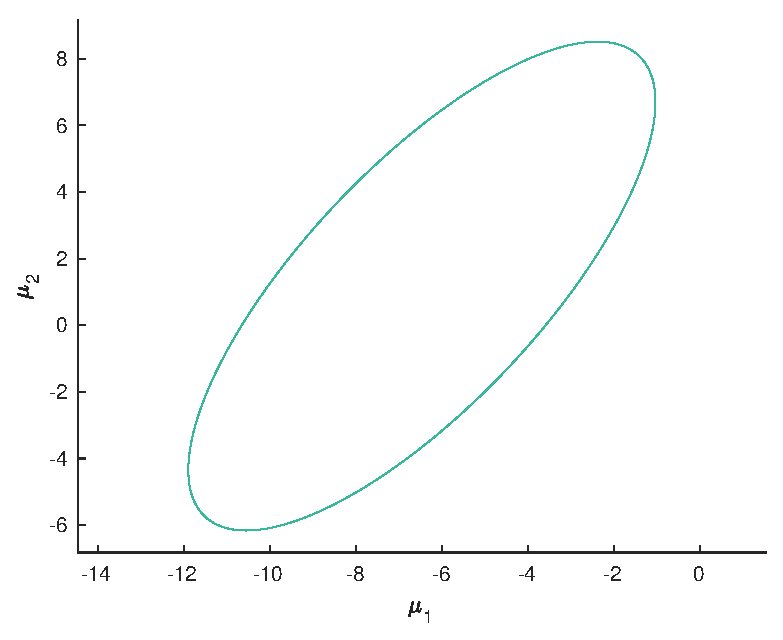
\includegraphics[width=10cm]{ex2fig}
  \caption{The confidence region of the difference
    $\b \mu_{\rm male} - \b \mu_{\rm female}$ with confidence 95\%. }
  \label{fig:ex2fig}
\end{figure}
The simultaneous confidence interval are $\b \mu = \b \mu_{\rm male}- \b
\mu_{\rm female}$ then we get that the confidence region for $\mu_{1}$
is given by 
\begin{equation*}
  \begin{pmatrix}
   -11.90 &-1.03  
  \end{pmatrix}
\end{equation*}
and, for $\mu_{2}$, 
\begin{equation*}
  \begin{pmatrix}
   -6.16 &8.52  
  \end{pmatrix}.
\end{equation*}
The confidence intervals ''frames'' the confidence region, as is shown
in Figure \ref{fig:ex2_sim_intervals}. 
\begin{figure}[h]
  \centering
  \includegraphics[width=10cm]{ex2fig_with_sim_intervals}
  \caption{Confidence region with and the simultaneous $T^{2}$-intervals plotted. }
  \label{fig:ex2_sim_intervals}
\end{figure}
\subsection*{(f)}
\label{sec:f}
There is evidence for that female birds have longer tails. However,
there is no significant difference between the genders when it comes to
the length of their wingspan. 


%%% Local Variables:
%%% mode: latex
%%% TeX-master: "examination"
%%% End:


\section*{Exercise 3}
\label{sec:exercise-3}

\subsection*{(a)}
\label{sec:a-2}
The plot of the profiles are presented in figure
\ref{fig:ex3-profiles}.
\begin{figure}[h]
  \centering
  \includegraphics[width=8.5cm]{ex3-profiles}
  \caption{The profiles for the Psychmotor scores given different
    radiation treatment.}
  \label{fig:ex3-profiles}
\end{figure}

\subsection*{(b)}
\label{sec:b-2}


Since we have more than tho profiles we wich to test, we have to use
the more general approach. Set up the variables as descibed in Lectrure
6. We can test if the profiles are parallel using
\begin{equation*}
  \lambda_{H_1} = \frac{\det CVC^T}{\det( CVC^T  + CHC^T),}
\end{equation*}
and createing the test variables
\begin{equation*}
  test = -\left(n - \frac 12(k + p -1)\right) \ln \Lambda_{H_1},
\end{equation*}
which is $\chi^2((p-1)(k-1))$. We reject $H_1$ if test variable is
smaller then the critical point, 
\begin{equation*}
  c = \chi^2 _{0.95} ((p-1)(k-1)).
\end{equation*}
From matlab we get
\begin{equation*}
  test = -4.0443,
\end{equation*}
and
\begin{equation*}
    c = 12.5916.
\end{equation*}
Since we $test < c$, we can not reject $H_1$, the profiles are parallel.


\subsection*{(c)}
\label{sec:c-2}

Since, the profiles are parallel, we can set up a test for checking if
the profiles are on the same level. This can be done by using the test
\begin{equation*}
  \lambda_{H_2 | H_1} = \frac{\det(CVC^T + CHC^T)}{\det(CVC^T)}\frac{\det(V)}{\det(V+H)},
\end{equation*}
and creating the test variable 
\begin{equation*}
  F = \left(\frac{n-k - p +1}{k - 1}\right)\frac{1 - \lambda_{H_2 |H_1}}{\lambda_{H_2 | H_1}},
\end{equation*}
which we compare to the critical value
\begin{equation*}
  c = F_{0.95} (k-1, n - k - p +1).
\end{equation*}
We get
\begin{equation*}
  -10.8296 = F < c = 2.8451,
\end{equation*}
we can not reject $H_2 | H_1$, the profiles are on the same level.

\subsection*{(d)}
\label{sec:d-1}

Here, we use the test variables 
\begin{equation*}
  \lambda_{H_3 | H_1} = \frac{1}{1 + n \bar{\bf x}^T C^T (CVC^T +
    CHC^T)^-1C*\bar{\bf x}},
\end{equation*}
and create the test variable
\begin{equation*}
  test = \frac{n - p +1}{p - 1}\lambda_{H_3 |H_1},
\end{equation*}
which we compare to 
\begin{equation*}
  c = F_{0.95}(p-1, n-p+1).
\end{equation*}
We get
\begin{equation*}
  7.9361 = test > c = 3.2145.
\end{equation*}
So we get that we have to reject $H_3 | H_1$, the profiles are not
flat.

\section*{\texttt{matlab} code}
\label{sec:textttmatlab-code}

\lstinputlisting[style=matlab]{../ex3.m}
%%% Local Variables:
%%% mode: latex
%%% TeX-master: "examination"
%%% End:


\section*{Exercise 4}
\label{sec:exercise-4}

\subsection*{(a)}
\label{sec:a-3}

We can check if the matrices can be pooled by using the test variable
\begin{equation*}
  \lambda^* = \frac{\Pi \det(V_i ^{f_i/2})}{\det(V^{f/2})}
  \frac{f^{pf/2}}{\Pi f_i ^{pfi/2}}
\end{equation*}
and using the Box correction, we get
\begin{equation*}
  -2  \frac{m}{f} \ln \lambda^* = 49.2750,
\end{equation*}
which we comapre against the critical value
\begin{equation*}
  c = \chi^2_{0.95}(f) = 58.1240,
\end{equation*}
hence the covariance matrices can be pooled into one matrix.

\subsection*{(b)}
\label{sec:b-3}

We could calculate the linear seprators, $ l_i^T x_0 + c_i$, where
we obtain
\begin{align*}
l_1^T x_0 + c_1 &= (-0.57, 1.80, 1.01, 6.33, 18.94, 0.33)x_0 + -703.95 \\ 
l_2^T x_0 + c_2 &= (-0.14, 1.31, 1.48, 5.15, 18.31, 0.04)x_0 + -554.06 \\ 
l_3^T x_0 + c_3 &= (-1.08, 1.89, 3.03, 5.69, 15.11, 0.51)x_0 + -618.43,
\end{align*}
In which we can conclude that ${\bf x_0}$ belongs to  $\pi_i$ if $
  l_i^T x_0 + c_i = \max_i \left(   l_i^T x_0 + c_i\right)
$

\subsection*{(C)}
\label{sec:c-3}

Since we have unkwn mean and variance, we use the approximation 
\begin{align*}
  e_1 &= \phi(\Delta) \frac{\Delta^2 + 12(p-1)}{16\Delta} \\
  e_2 &=  \phi(\Delta)\frac{\Delta^2 - 4(p-1)}{16\Delta},
\end{align*}
where $\Delta$,  $a_1$ and $a_2$  are defined as in the lectures.
Using the pooled matrix $S_p$ for all three populations, we got the
probablity of classifying wrongly into $\pi_1$ to be
\begin{equation*}
  e_1 \approx 0.0019
\end{equation*},
and for $\pi_2$ to be
\begin{equation*}
  e_2  \approx 0.0019.
\end{equation*}
\subsection*{Code}
\label{sec:code}



\lstinputlisting[style=matlab]{./../ex4.m}
%%% Local Variables:
%%% mode: latex
%%% TeX-master: "examination"
%%% End:


\printbibliography

\end{document}
%%% Local Variables:
%%% mode: latex
%%% TeX-master: t
%%% End:
